\subsection{Công cụ sử dụng}\label{cong-cu-su-dung}

\subsubsection{Linux}\label{linux}

Môi trường thực hiện sử dụng Linux/Proxmox làm nền tảng triển khai và kiểm thử Docker, Docker Bench Security, Ansible, Prometheus và Grafana.

\subsubsection{Docker Bench Security}\label{docker-bench-security}

\begin{quote}
Docker Bench Security là một script mã nguồn mở do Docker Inc. phát triển. Công cụ này tự động kiểm tra các Benchmark theo chuẩn CIS Docker Benchmark trên môi trường Docker đang chạy, cho phép quản trị viên nhanh chóng đánh giá mức độ tuân thủ bảo mật của hệ thống.

Docker Bench Security hoạt động bằng cách mount các thư mục hệ thống của host vào container kiểm tra, sau đó thực thi các bài kiểm tra tương ứng với từng Section trong CIS Docker Benchmark. Với mỗi mục kiểm tra, công cụ trả về một trong ba kết quả:
\end{quote}

\begin{itemize}
\item
  PASS: Cấu hình hiện tại đáp ứng đúng khuyến nghị.
\item
  WARN: Cấu hình không đáp ứng khuyến nghị, cần khắc phục.
\item
  INFO: Thông tin bổ sung, cần xem xét thủ công.
\end{itemize}

\begin{quote}
Kết quả được xuất ra terminal và lưu đồng thời vào hai file log: docker-bench- security.log (dạng văn bản) và docker-bench-security.log.json (dạng JSON) để phục vụ phân tích hoặc tích hợp vào pipeline CI/CD.

Tool này sẽ được sử dụng để đối chứng kết quả với audition tự làm và cho việc remediation.
\end{quote}

Docker Bench Security https://github.com/docker/docker-bench-security\protect\phantomsection\label{_bookmark25}{}

\subsubsection{Ansible}\label{ansible}

\begin{quote}
Sử dụng Ansible để tự động hóa và cải thiện Docker phù hợp với Benchmark sau khi thực hiện manual:
\end{quote}

\begin{itemize}
\item
  Host: Đích đến sẽ là Docker
\item
  Các file yaml/yml sẽ là các mục từ 1 đến 6.
\end{itemize}

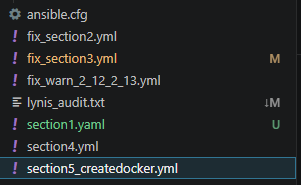
\includegraphics[width=3.13585in,height=1.92735in]{images/media/image3.png}
